\section{Educational DP Contest}

\subsection{A - Frog 1}
\begin{framed}
    有$N$块石头,编号为$1, 2, \ldots, N$。每块$i$($1 \leq i \leq N$),石头$i$的高度为$h_i$。

    有一只青蛙,它最初在石块 $1$ 上。它会重复下面的动作若干次以到达石块$N$:
    \begin{itemize}
        \item 如果青蛙目前在石块$i$上,则跳到石块$i + 1$或石块$i + 2$上。这里需要付出$|h_i - h_j|$的代价,其中$j$是要降落的石块。
    \end{itemize}

    求青蛙到达石块$N$之前可能产生的最小总成本。
\end{framed}
简单的线性dp,$f[i]$为到达$i$的最小的代价,所以转移方程就是:

$f[i]=\min( f[i-1] - |h_i-h_{i-1}|,f[i-2]-|h_i-h_{i-2}|)$
\lstinputlisting{动态规划/Educational DP Contest/A.cpp}

\subsection{B - Frog 2}
\begin{framed}
    有$N$块石头,编号为$1, 2, \ldots, N$。每块$i$($1 \leq i \leq N$),石头$i$的高度为$h_i$。

    有一只青蛙,它最初在石块 $1$ 上。它会重复下面的动作若干次以到达石块$N$:
    \begin{itemize}
        \item 如果青蛙目前在石块$i$上,请跳到以下其中一个位置:石块$i + 1, i + 2, \ldots, i + K$。这里会产生$|h_i - h_j|$的代价,其中$j$是要降落的石头。
    \end{itemize}
    求青蛙到达石块$N$之前可能产生的最小总成本。
\end{framed}
与上一题不同的是,这次转移的前驱很多,但依旧可以直接转移,复杂度$O(NK)$
\lstinputlisting{动态规划/Educational DP Contest/B.cpp}

\subsection{C - Vacation}
\begin{framed}
    有 $N$ 天。每$i$ ($1 \leq i \leq N$)天,第$i$天有三种活动$A,B,C$,只能进行一种活动,每种活动会获得$a_i,b_i,c_i$的快乐值,相邻两天的活动不能相同,请求快乐值之和的最大值。
\end{framed}
$f[i][j]$表示前$i$天,且第$i$天进行活动$j$的最大快乐值。只需要$3\times 3$ 的枚举状态和前驱进行转移即可。
\lstinputlisting{动态规划/Educational DP Contest/C.cpp}

\subsection{D - Knapsack 1}
\begin{framed}
    有 $N$ 个项目,编号为 $1, 2, \ldots, N$。对于每个$i$($1 \leq i \leq N$),项目$i$的权重为$w_i$,值为$v_i$。

    太郎决定从$N$件物品中选择一些装进背包里带回家。背包的容量为 $W$,这意味着所取物品的权重之和最多为 $W$。

    求太郎带回家的物品价值的最大可能和。
\end{framed}
01背包
\lstinputlisting{动态规划/Educational DP Contest/D.cpp}

\subsection{E - Knapsack 2}
\begin{framed}
    有 $N$ 个项目,编号为 $1, 2, \ldots, N$。对于每个$i$($1 \leq i \leq N$),项目$i$的权重为$w_i$,值为$v_i$。

    太郎决定从$N$件物品中选择一些装进背包里带回家。背包的容量为 $W$,这意味着所取物品的权重之和最多为 $W$。

    求太郎带回家的物品价值的最大可能和。
\end{framed}
还是 01 背包,但是本题中$W$范围非常大,无法枚举。这也用到了一个常用的优化思路,考虑$N\times v_i\le 10^5$,所以可以背包求出价值为$i$的最小代价,然后找到合法的最大值即可。
\lstinputlisting{动态规划/Educational DP Contest/E.cpp}

\subsection{F - LCS}
\begin{framed}
    给你字符串 $s$ 和 $t$。请找出一个最长的字符串,它同时是 $s$ 和 $t$ 的子串。
\end{framed}
典题求 LCS 并还原。
\lstinputlisting{动态规划/Educational DP Contest/F.cpp}

\subsection{G - Longest Path}
\begin{framed}
    有一个有向图$G$,它有$N$个顶点和$M$条边。顶点编号为 $1, 2, \ldots, N$,对于每个 $i$ ($1 \leq i \leq M$),$i$条有向边从顶点 $x_i$ 到 $y_i$。$G$不包含有向循环。

    求$G$中最长有向路径的长度。这里,有向路径的长度就是其中边的数量。
\end{framed}
因为不存在有向环,所以最长的路径起点一定入度为 0,终点一定出度为 0。想到这个结论后,比较容易想的就是在拓扑序上线性递推即可。
\lstinputlisting{动态规划/Educational DP Contest/G.cpp}

\subsection{H - Grid 1}
\begin{framed}
    有一个网格,横向有 $H$ 行,纵向有 $W$ 列。让 $(i, j)$ 表示从上往下第 $i$ 行和从左往上第 $j$ 列的正方形。

    对于每个$i$和$j$($1 \leq i \leq H$,$1 \leq j \leq W$),方格$(i, j)$由一个字符$a_{i, j}$来描述。如果 $a_{i, j}$ 是 `.`,则方格 $(i, j)$ 是一个空方格;如果 $a_{i, j}$ 是 `#`,则方格 $(i, j)$ 是一个墙方格。可以保证方格$(1, 1)$和$(H, W)$是空方格。

    太郎会从方格$(1, 1)$开始,通过反复向右或向下移动到相邻的空方格,到达$(H, W)$。

    求太郎从$(1, 1)$到$(H, W)$的路径数。由于答案可能非常大,请求取$10^9 + 7$的模数。
\end{framed}
简单的二维转移
\lstinputlisting{动态规划/Educational DP Contest/H.cpp}

\subsection{I - Coins}
\begin{framed}
    设 $N$ 是一个正奇数。

    有 $N$ 枚硬币,编号为 $1, 2, \ldots, N$。对于每个 $i$ ($1 \leq i \leq N$),当抛掷硬币 $i$ 时,正面出现的概率为 $p_i$,反面出现的概率为 $1 - p_i$。

    太郎抛出了所有的 $N$ 枚硬币。求正面比反面多的概率。
\end{framed}
简单的概率 dp,设$f[i][j]$表示前$i$个硬币$j$个正面的个数,转移如下:
$$
f[i][j]=f[i-1][j-1]\times p_i + f[i-1][j] \times (1 - p_i)
$$
显然可以通过倒序枚举优化掉一维空间。

答案就是$\sum (f[n][i] \times( i > n - i ))$

\lstinputlisting{动态规划/Educational DP Contest/I.cpp}

\subsection{J - Sushi}
\begin{framed}
    有$N$道菜,编号为$1, 2, \ldots, N$。最初,每个$i$($1 \leq i \leq N$),$i$盘都有$a_i$($1 \leq a_i \leq 3$)个寿司。($1 \leq a_i \leq 3$) 块寿司。

    太郎会重复执行以下操作,直到所有寿司都被吃掉:

    掷一个骰子,骰子上显示的数字$1, 2, \ldots, N$的概率相等,结果为$i$。如果骰子$i$上有几块寿司,就吃掉其中一块;如果没有,就什么都不吃。

    求在所有寿司都被吃掉之前进行该操作的预期次数。
\end{framed}

可以注意到的是选择哪个盘子无所谓,答案与盘子的顺序无关,只与盘子中剩下寿司数量有关。

可以设状态为$f[a][b][c]$表示当前有$a$个盘子剩1 个,$b$个盘子剩 2 两个,$c$个盘子剩三个的期望操作次数。

则有$\frac a n$的概率选择剩 1 个的盘子,$\frac b n $的概率选到剩 2 个的盘子,$\frac c n$的概率选到剩 3 个的盘子,$\frac {n-a-b—c}{n}$的概率选到剩 0 个的盘子。

所以转移方程为
$$
f[a][b][c] = 1 + \frac{a}{n} f[a-1][b][c] + \frac{b}{c} f[a+1][b-1][c] +\frac{c}{n}f[a][b+1][c] + \frac{n-a-b-c}{n} f[a][b][c]
$$
可以看到$f[a][b][c]$出现在了方程两侧,所以可以把方程移项得到
$$
f[a][b][c] = \frac {n}{ a+b+c} + \frac{a}{a+b+c} f[i-1][j][k] + \frac{b}{a+b+c}f[a+1][b-1][c] +\frac{c}{a+b+c} f[a][b+1][c-1]
$$
根据这个方程便可以进行转移,但枚举比较复杂,所以可以使用深搜加记忆化实现代码
\lstinputlisting{动态规划/Educational DP Contest/J.cpp}

\subsection{K - Stones}
\begin{framed}
    有一个由 $N$ 个正整数组成的集合 $A = \{ a_1, a_2, \ldots, a_N \}$。太郎和二郎将进行下面的对弈。

    最初,我们有一堆由 $K$ 个石子组成的棋子。从太郎开始,两位棋手交替进行以下操作:

    在$A$中选择一个元素$x$,然后从棋子堆中移走正好$x$个棋子。

    当棋手无法下棋时,他就输了。假设两位棋手都以最佳状态下棋,请确定获胜者。
\end{framed}
如果当前没有石子,则为先手必败态。所有能够一步到达先手必败的状态均为先手必胜态,无论如何都到达不了先手必败态的状态就是先手必败态。
\lstinputlisting{动态规划/Educational DP Contest/K.cpp}

\subsection{L - Deque}
\begin{framed}
    太郎和二郎将进行以下对弈。

    最初,他们得到一个序列 $a = (a_1, a_2, \ldots, a_N)$。在 $a$ 变为空之前,两位棋手从太郎开始交替执行以下操作:

    移除 $a$ 开头或结尾的元素。棋手获得$x$分,其中$x$为移除的元素。

    假设$X$和$Y$分别是太郎和二郎在游戏结束时的总得分。太郎试图最大化$X - Y$,而二郎试图最小化$X - Y$。

    假设两位棋手的下法都是最优的,请找出$X - Y$的结果值。
\end{framed}

设$f[l][r][1]$表示区间$[l,r]$中$X-Y$的最大值且最后一次操作是太郎,$f[l][r][0]$表示区间$[l,r]$中$Y-X$的最大值二郎,所以转移如下:

$
f[l][r][1] = \max( a[l] - f[l+1][r][0] , a[r] - f[l][r-1][0])

\\f[l][r][0] = \max( a[r] - f[l+1][r][0] , a[r] - f[l][r-1][0])
$

然后发现两个方程的转移是完全一样的,且最终得到的结果也是一样的,所以可以省略掉第三位。

\lstinputlisting{动态规划/Educational DP Contest/L.cpp}

\subsection{M - Candies}
\begin{framed}
    有$N$个孩子,编号为$1, 2, \ldots, N$。

    他们决定分享$K$颗糖果。在这里,每个$i$($1 \leq i \leq N$),$i$个孩子必须分到$0$到$a_i$颗糖果(包括$0$和$a_i$)。另外,糖果不能剩下。

    求他们分享糖果的方法数,模数为 $10^9 + 7$。在这里,如果有一个孩子得到的糖果数量不同,那么这两种方法就是不同的。
\end{framed}
前缀和优化。

首先$dp[i][j]$表示前$i$个人共分得$j$个糖果的方案数。下一个套路就是枚举第$i$个人分到的多少糖果,但是这样做复杂度太高了,转移如下
$$
dp[i][j] = \sum_{k=\max(j-a[i],0)}^{j} dp[i-1][k]
$$
如果我们维护出了$dp[i-1][k]$的前缀和,这就可以省掉一维的枚举。
\lstinputlisting{动态规划/Educational DP Contest/M.cpp}

\subsection{N - Slimes}
\begin{framed}
    有 $N$ 个黏液排成一排。最初,左边的 $i$ 个黏液的大小是 $a_i$ 。

    太郎正试图将所有的黏液组合成一个更大的黏液。他会反复执行下面的操作,直到只有一个粘液为止:

    选择两个相邻的粘液,将它们组合成一个新的粘液。新黏液的大小为 $x + y$ ,其中 $x$ 和 $y$ 是合并前黏液的大小。这里需要花费 $x + y$ 。在组合粘泥时,粘泥的位置关系不会改变。

    求可能产生的最小总成本。
\end{framed}
区间dp模板。

$f[l][r]$表示区间把$[l,r]$合并的最小代价。

我们枚举出$[l,r]$然后枚举出分界点$mid$,然后可以转移
$$
f[l][r]=f[l][mir] + f[mid+1][r] +\sum a_i
$$
所以我们枚举区间的时候必须要从小到大。
\lstinputlisting{动态规划/Educational DP Contest/N.cpp}

\subsection{O - Matching}
\begin{framed}
    有 $N$ 名男性和 $N$ 名女性,编号均为 $1, 2, \ldots, N$ 。

    对于每个 $i, j$ ( $1 \leq i, j \leq N$ ),男人 $i$ 和女人 $j$ 的相容性都是一个整数 $a _{i, j}$ 。如果是 $a_{i, j} = 1$ ,则男人 $i$ 和女人 $j$ 相容;如果是 $a _ {i, j} = 0$ ,则不相容。

    太郎试图做出 $N$ 对,每对都由一个相容的男人和一个相容的女人组成。在这里,每个男人和每个女人必须正好属于一对。

    求太郎能凑成 $N$ 对的方式数,模为 $10^9 + 7$ 。
\end{framed}
简单的状压 dp,设状态为$f[i][t]$表示前$i$个男生,匹配女生状态$t$的方案数,其中$t$是一个二进制数每一位 01 表示一位女生是否完成匹配。每次只要枚举状态,然后再枚举当前男生和哪一位女生匹配即可计算出前驱状态。
\lstinputlisting{动态规划/Educational DP Contest/O.cpp}

\subsection{P - Independent Set}
\begin{framed}
    有一棵树,树上有 $N$ 个顶点,编号为 $1, 2, \ldots, N$ 。对于每个 $i$ ( $1 \leq i \leq N - 1$ ), $i$ -th 边连接顶点 $x_i$ 和 $y_i$ 。

    太郎决定将每个顶点涂成白色或黑色。这里不允许将相邻的两个顶点都涂成黑色。

    求 $10^9 + 7$ 模中可以涂抹顶点的方法的个数。
\end{framed}
树形 dp,$f[i][0/1]$表示$i$好的白或黑的方案数,然后我们可以枚举子节点,要知道白色的子节点黑白任意,黑色的子节点只有黑色。
\lstinputlisting{动态规划/Educational DP Contest/P.cpp}

\subsection{Q - Flowers}
\begin{framed}
    有 $N$ 朵花排成一排。对于每一朵 $i$ ( $1 \leq i \leq N$ ),从左边起第 $i$ 朵花的高和美分别是 $h_i$ 和 $a_i$ 。这里, $h_1, h_2, \ldots, h_N$ 都是不同的。

    太郎正在拔掉一些花朵,以便满足以下条件:

    剩余花朵的高度从左到右单调递增。

    求剩余花朵的美之和的最大值。
\end{framed}
发现高度的值域其实很小,所以可以设状态为$f[i][j]$表示前$i$朵花,且最大高度不超过$j$的美之和最大值。则有转移如下
\[
    f[i][j] = \max_{k=0}^{h[i]}( f[i-1][k]) + a[i]
\]
然后很容易就可以压缩掉一维,然后转移就变成求前缀最大值。求前缀最大值可以用树状数组实现。
\lstinputlisting{动态规划/Educational DP Contest/Q.cpp}

\subsection{R - Walk}
\begin{framed}
    有一个简单的有向图 $G$ ,其顶点为 $N$ ,编号为 $1, 2, \ldots, N$ 。

    对于每个 $i$ 和 $j$ ( $1 \leq i, j \leq N$ ),你都会得到一个整数 $a_{i, j}$ ,表示顶点 $i$ 到 $j$ 之间是否有一条有向边。如果是 $a_{i, j} = 1$ ,则存在一条从顶点 $i$ 到 $j$ 的有向边,如果是 $a_{i, j} = 0$ ,则没有。

    求在 $G$ 中长度为 $K$ 的不同有向路径的数目,模数为 $10^9 + 7$ 。我们还将计算多次穿越同一条边的路径。
\end{framed}

我们设$f_i[x][y]$表示长度为$i$且从$x$到$y$的路径的方案数,则输入的矩阵就是$f_1$。然后我们根据传递闭包得到转移如下
\[
    f_i[x][y] = \sum_{k=1}^n f_{i-1}[x][k] \times f_1[k][y]
\]
很容易发现这个转移过程就是矩阵乘法
\[
    f_i = f_{i-1}\times f_1
\]
所以可以用矩阵快速幂来解决这个问题。
\lstinputlisting{动态规划/Educational DP Contest/R.cpp}

\subsection{S - Digit Sum}
\begin{framed}
    求在 $1$ 和 $K$ (含)之间满足以下条件的整数个数,模为 $10^9 + 7$ :

    十进制数位之和是 $D$ 的倍数。
\end{framed}
$f[pos][x]$表示前$pos$位和模$d$为$x$的数的个数。

然后我们设$dp(pos,x,flag)$,其中$flag$表示前$pos$是否完全与原数相同。如果相同则当前位的取值是$[0,a[pos]]$否则是$[0,9]$。然后枚举当前位更新状态即可。

注意如果前$pos$位不与原数完全相同是,要用记忆化。
\lstinputlisting{动态规划/Educational DP Contest/S.cpp}

\subsection{T - Permutation}
\begin{framed}
    设 $N$ 是一个正整数。给你一个长度为 $N - 1$ 的字符串 $s$ ,由 $<$ 和 $>$ 组成。

    求满足以下条件的 $(1, 2, \ldots, N)$ 的 $(p_1, p_2, \ldots, p_N)$ 排列的个数,模数为 $10^9 + 7$ :

    对于每个 $i$ ( $1 \leq i \leq N - 1$ ),如果 $s$ 中的 $i$ -th 字符是 $<$,则为 $p_i \lt p_{i + 1}$ ;如果 $s$ 中的 $i$ -th 字符是 $>$,则为 $p_i \gt p_{i + 1}$ 。
\end{framed}
设状态为$f[i][j]$表示$[1,i]$的排列,且最后一位是$j$的方案数。

如果符号是$<$,则$f[i][j] = \sum_{t = 1} ^{j-1} f[i-1][t]$

如果符号是$>$,则$f[i][j] = \sum_{t=j}^{i} f[i-1][t]$

这样如果维护了一个前缀和就可以$O(1)$的进行转移了。
\lstinputlisting{动态规划/Educational DP Contest/T.cpp}

\subsection{U - Grouping}
\begin{framed}
    有 $N$ 只兔子,编号为 $1, 2, \ldots, N$ 。

    对于每只 $i, j$ ( $1 \leq i, j \leq N$ ),兔子 $i$ 和 $j$ 的兼容性用整数 $a_{i, j}$ 来描述。这里, $a_{i, i} = 0$ 表示每个 $i$ ( $1 \leq i \leq N$ ), $a_{i, j} = a_{j, i}$ 表示每个 $i$ 和 $j$ ( $1 \leq i, j \leq N$ )。

    太郎要把 $N$ 只兔子分成若干组。在这里,每只兔子必须正好属于一组。分组后,对于每只 $i$ 和 $j$ ( $1 \leq i \lt j \leq N$ ),如果兔子 $i$ 和 $j$ 属于同一组,太郎就能获得 $a_{i, j}$ 分。

    求太郎可能得到的最高总分。
\end{framed}
设$f[s]$表示当前选择选择的兔子集合为$s$的最高总分,获得总分只有两种情况,一种是$s$所有的兔子在一组中。还有一种是$s$由至少两个组拼起来的。

对于只有一组的情况,直接统计一下就好,对于多个组拼起来的则使用枚举的子集的方式来求。
\lstinputlisting{动态规划/Educational DP Contest/U.cpp}

\subsection{V - Subtree}
\begin{framed}
    给一棵树,对每一个节点染成黑色或白色。

    对于每一个节点,求强制把这个节点染成黑色的情况下,所有的黑色节点组成一个联通块的染色方案数,答案对 $M$ 取模。
\end{framed}
换根 dp。

首先可以任意选择一个点做根节点,我代码里面选择的是$1$,选定根节点后,树就变成了一颗有根树。

现在对于每个点$x$,如果知道了子树中的合法方案数$f1[x]$和非子树节点的合法方案数$f2[x]$,则答案就是$f1[x] \times f2[x]$

考虑求$f1[x]$,我们可以枚举$x$的子节点$y$,则有如下转移
\[
    f1[x] = \Pi (f1[y] + 1)
\]
然后考虑如何求$f2[x]$,我们已知了$x$的父亲节点$fa$和兄弟节点$y$,则有如下转移
\[
    f2[x] = f2[fa] \times\Pi (f1[y] + 1) + 1
\]
其中如果要求解$\Pi(f1[y]+1)$的话复杂度是$O(N^2)$的,这里因为要取模,所以采用了前缀积和后缀积的方法,$pre[y]$表示$y$前面兄弟结点的前缀积,$suf[y]$表示$y$后面兄弟节点的后缀积,则$f2[x] = f2[fa]\times pre[x]\times suf[x] + 1$
\lstinputlisting{动态规划/Educational DP Contest/V.cpp}

\subsection{W - Intervals}
\begin{framed}
    给定 $m$ 条规则形如 $(l_i,r_i,a_i)$,对于一个 01 串,其分数的定义是:对于第 $i$ 条规则,若该串在 $[l_i,r_i]$ 中至少有一个 1,则该串的分数增加 $a_i$。

    你需要求出长度为 $n$ 的 01 串中的最大分数。

    $1\le n,m\le 2\times 10^5$,$|a_i|\le 10^9$。
\end{framed}
线段树优化 dp。

设$f[i][j]$表示前$i$个位置,且最后一个$1$的位置为$j$的最大分数。并且我们强制规定,对于$(l_k,r_k,a_k)$我们只考虑$r_k\le i$的贡献。显然这里有一个合法条件一定是$j\le i$,所以有如下的转移
\[
    f[i][j] = \left\{\begin{matrix}
                         \max_{1\le l < i}(f[i-1][l]) + \sum_{l_k\le j \and r_k=i }a_k & j = i \\
                         f[i-1][j] + \sum_{l_k\le j \and r_k = i} a_k                  & j < i
    \end{matrix}\right.
\]
为什么有这样的转移呢?首先如果$j<i$则前$i-1$位的最后一个也一定是$j$,如果$j = i $则前面的最后一位是可以任意取的。

然后我们发现对于第一维只和上一位有关,所以可以优化掉一维空间。

然后我们发现转移可以分为两部分。

第一部分是$f[i] = \max( f[j] )$。

第二部分是对于所有满足$r_k=i$的$(l_k,r_k,a_k)$,都有$ f[j] = f[j] + a_k , (l_k\le j \le r_k)$。

对于这两部分操作,实际上就是区间最值查询和区间修改,可以使用线段树来实现。
\lstinputlisting{动态规划/Educational DP Contest/W.cpp}

\subsection{ X - Tower}
\begin{framed}
    有 $N$ 块,编号为 $1, 2, \ldots, N$ 。对于每个 $i$ ( $1 \leq i \leq N$ ),积木块 $i$ 的重量为 $w_i$ ,坚固度为 $s_i$ ,价值为 $v_i$ 。

    太郎决定从 $N$ 块中选择一些,按照一定的顺序垂直堆叠起来,建造一座塔。在这里,塔必须满足以下条件:

    - 对于塔中的每个积木块 $i$ ,堆叠在其上方的积木块的权重之和不大于 $s_i$ 。

    求塔中所包含的图块的最大可能权重之和。
\end{framed}
这道题算是贪心优化 dp。

首先考虑什么样的更适合放在下面?如果$i$比$j$更适合放在下面,则$s_i-w_k> s_j-w_i$也就可以化简得到$s_i+w_i > s_j + w_j$。这样可以进行一个排序,从小到大排序。

然后我们考虑从上往下放$f[i]$表示当前累计重量为$i$的最大价值。现在如果枚举到了物品$j$则有如下转移
\[
    f[j+w_i] = \max( f[j+w_i] , f[i] + v[i] )
\]
其中$j\le s_i$,这样就可以转化成经典的 01 背包问题,记得使用倒序枚举。
\lstinputlisting{动态规划/Educational DP Contest/X.cpp}

\subsection{Y - Grid 2}
\begin{framed}
    给一个 $H\times W$ 的网格,每一步只能向右或向下走,给出 $N$ 个坐标 $(r_1,c_1),(r_2,c_2),...,(r_n,c_n)$,这些坐标对应的位置不能经过,求从左上角 $(1,1)$ 走到右下角 $(H,W)$ 的方案数,答案对 $10^9+7$ 取模。

    $2 \leq H, W \leq 10^5 ,1 \leq N \leq 3000$
\end{framed}
首先从一个点到$(x_1,y_1)$到$(x_2,y_2)$的路径数有$C(x_1 + y_1 - x_2 - y_2 , x_1 - x_2)$中。

记从$(1,1)$到$(x_i,y_i)$不经过任何障碍物的路径数$f[i]$,则有如下转移
\[
    f[i] = C(x_i + y_i - 2 , x_i - 1 ) - \sum f[j] \times C( x_i + y_i - x_j - y_j , x_i - x_j)
\]
其中$j$是比$i$更靠近起点的点。看起来是容斥掉了一个点,让实际上因为我们记录的是不经过任何障碍物的路径,所以容斥的时候是不会重复容斥的。
\lstinputlisting{动态规划/Educational DP Contest/Y.cpp}

\subsection{Z - Frog 3}
\begin{framed}
    有 $N$ 块石头,编号为 $1, 2, \ldots, N$ 。每块 $i$ ( $1 \leq i \leq N$ )石头 $1 \leq i \leq N$ ),石头 $i$ 的高度为 $h_i$ 。这里, $h_1 \lt h_2 \lt \cdots \lt h_N$ 成立。

    有一只青蛙,它最初位于石块 $1$ 上。它会重复下面的动作若干次以到达石块 $N$ :

    - 如果青蛙目前在 $i$ 号石块上,请跳到以下其中一块:石块 $i + 1, i + 2, \ldots, N$ 。这里需要花费 $(h_j - h_i)^2 + C$ ,其中 $j$ 是要落脚的石头。

    求青蛙到达石块 $N$ 之前可能产生的最小总成本。

    $2 \leq N \leq 2 \times 10^5$
\end{framed}
斜率优化 dp。

设$f[i]$表示从$1$到$i$的最小花费,这可以写出最基础的状态转移为
$$
f[i] = \min( f_j + (h_i-h_j)^2 + C)
$$
内部可以展开为
$$
f[i] = \min( f_j h_i^2 + h_j^2 + C - 2h_ih_j)
$$
把无关项提出来,可以得到
$$
f[i] = h_i^2 + C + min( f_j + h_j^2 - 2h_ih_j )
$$
令$g_i = f_i + h_i^2$,则有
$$
f[i] = h_i + C + min( g_j - 2h_ih_j)
$$
至此,关于式子的化简就结束了,现在对于转移,如果有两个点$x,y$,若满足$x<y$且$x$更优,则有
$$
g_x - 2h_ih_x < g_y - 2h_ih_y
$$
移项得
$$
\frac{g_x-g_y}{h_x - h_y} > 2h_i
$$
发现这个式子和斜率很像,所以令$slop(x,y)=\frac{g_x-g_y}{h_x - h_y}$。

下面就开始时斜率优化的部分,有三个点$1<2<3$,如果$2$是最优的则有
$$
slop(1,2) < 2h_i \and slop(2,3) > 2h_i \Rightarrow slop(1,2) < slop(2,3)
$$
对于下图

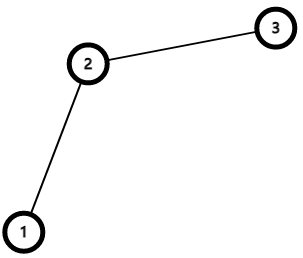
\includegraphics{动态规划/Educational DP Contest/11.png}

发现$slop(1,2)>slop(2,3)$,因此$2$一定不是最优的,所以可以优化成

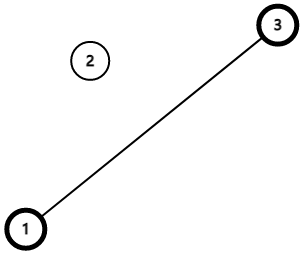
\includegraphics{动态规划/Educational DP Contest/22.png}

最后你会发现,实际上就是维护一个凸包

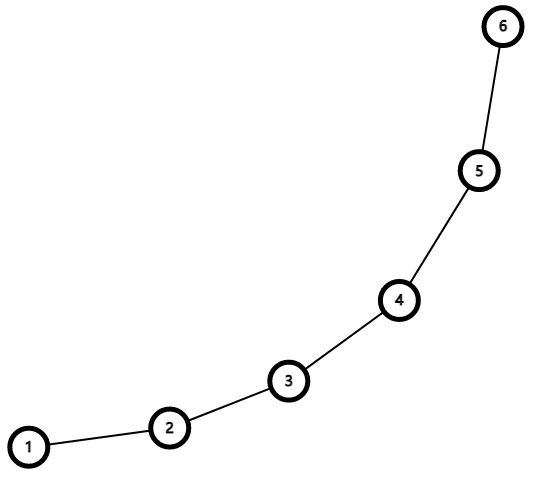
\includegraphics{动态规划/Educational DP Contest/33.png}

然后,因为本题的$h_i$时保证递增的,所以最优解只会出现在队首
\lstinputlisting{动态规划/Educational DP Contest/Z.cpp}